\documentclass[aspectratio=169]{beamer}

\usetheme{Madrid}
\definecolor{ftteal}{RGB}{13,148,136}
\definecolor{ftindigo}{RGB}{79,70,229}
\setbeamercolor{structure}{fg=ftteal}
\setbeamercolor{palette primary}{bg=ftteal, fg=white}
\setbeamercolor{palette secondary}{bg=ftteal!80!black, fg=white}
\setbeamercolor{palette tertiary}{bg=ftindigo, fg=white}
\setbeamercolor{title}{bg=ftteal, fg=white}
\setbeamertemplate{navigation symbols}{}

\usepackage{amsmath}
\usepackage{graphicx}
\usepackage{booktabs}
\usepackage{tikz}

\title[Short Title]{Presentation Title}
\subtitle{An optional subtitle}
\author[Your Name]{Your Name}
\institute[MMU]{Faculty of Computing and Informatics\\Multimedia University}
\date{\today}

\AtBeginSection[]{
  \begin{frame}
    \frametitle{Outline}
    \tableofcontents[currentsection]
  \end{frame}
}

\begin{document}

\begin{frame}
  \titlepage
\end{frame}

\begin{frame}{Outline}
  \tableofcontents
\end{frame}

\section{Introduction}

\begin{frame}{Motivation}
  \begin{itemize}
    \item<1-> Point one appears first
    \item<2-> Point two appears on the next click
    \item<3-> Point three appears last
  \end{itemize}
\end{frame}

\begin{frame}{Blocks}
  \begin{block}{A standard block}
    Use blocks to highlight key ideas.
  \end{block}
  \begin{alertblock}{An alert block}
    Draw attention to important warnings.
  \end{alertblock}
  \begin{exampleblock}{An example block}
    Show worked examples.
  \end{exampleblock}
\end{frame}

\section{Method}

\begin{frame}{Two Columns}
  \begin{columns}[T]
    \begin{column}{0.5\textwidth}
      \textbf{Left column}
      \begin{itemize}
        \item Text on the left
        \item More text
      \end{itemize}
    \end{column}
    \begin{column}{0.5\textwidth}
      \centering
      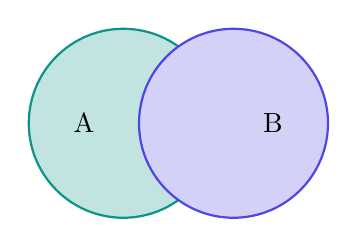
\begin{tikzpicture}
        \draw[fill=ftteal!25, draw=ftteal, thick] (0,0) circle (1.2);
        \draw[fill=ftindigo!25, draw=ftindigo, thick] (1.4,0) circle (1.2);
        \node at (-0.5,0) {A};
        \node at (1.9,0) {B};
      \end{tikzpicture}
    \end{column}
  \end{columns}
\end{frame}

\begin{frame}{Mathematics}
  The quadratic formula:
  \[
    x = \frac{-b \pm \sqrt{b^2 - 4ac}}{2a}
  \]
  \pause
  Bayes' theorem:
  \[
    P(A \mid B) = \frac{P(B \mid A)\, P(A)}{P(B)}
  \]
\end{frame}

\section{Results}

\begin{frame}{Results}
  \centering
  \begin{tabular}{lcc}
    \toprule
    Model & Accuracy & Speed \\
    \midrule
    Baseline & 82\% & 1.0$\times$ \\
    Ours & \textbf{91\%} & 1.4$\times$ \\
    \bottomrule
  \end{tabular}
\end{frame}

\begin{frame}
  \centering
  \Huge Thank you!\\[1em]
  \large Questions?
\end{frame}

\end{document}
